\section{Proposed Framework} \label{sec:Technical}
The main objective of this work is to create a generic framework for Supply Chain Management (SCM). Árion project is divided into three main modules described below: Frond-End WebApp, Back-End WebApp and Data Storage. Figure~\ref{fig:detalhamentotecnico} shows the application architecture and its components.

A SCM platform relies on three main items: assets (the goods itself or a token related to it), steps (phases which products go through) and actors (people who transact assets during the steps). Our approach is based on this triad, that must be defined on creation of a new supply chain.

Initially, a configuration file in JSON format is generated and read in the Blockchain platform, adding the main information for the correct functioning of the chain. The mechanism for creating this configuration file is detailed in the Sections \Cref{sec:UserInteraction,sec:ServiceLayer}.

%htbp
\begin{figure*}[ht]
\begin{center}
  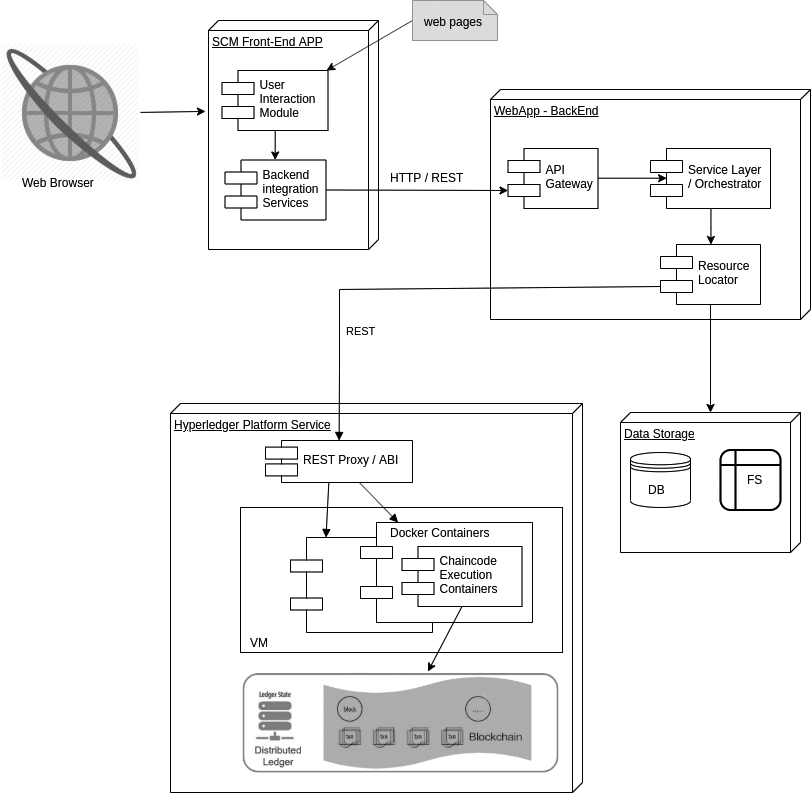
\includegraphics[scale=0.4]{images/detalhamentotecnico.png}
\caption{Árion Application architecture}
\label{fig:detalhamentotecnico}
\end{center}
\end{figure*}

\subsection{Frond-End WebApp}\label{sec:WebAppFrondEnd}
Front-End WebApp is a client–server application which the client (including the user interface and client-side logic) runs in a web browser. This is a single-page application (SPA) that interacts with the user by dynamically rewriting the current page rather than loading entire new pages from a server. The application is build with React (also known as React.js or ReactJS). The Front-End Webapp is divided into two main blocks and these are classified according to the interactions: User Interaction Modules and Backend Interaction Services.

\subsubsection{User Interaction Modules}\label{sec:UserInteraction}
User Interaction modules are responsible for providing web pages that will be rendered on client’s web browser. These interactions are provided by modules described below.

The Login Module is responsible for display the login and authentication alternatives pages (e.g. ‘forgot my password’, ‘reset my password’). The Application Configuration module provides the features of the creation/configuration of supply chain items and supply chain flows (steps). This module is responsible for getting the information from the user to generate the configuration JSON file in the backend. User handling module provides the features for the creation/configuration of Actors and Steps, complementing configuration file. The Data Entry module provides form pages that allow the actors to enter data in the application, search and move assets from a step to another. The Data Visualization module is responsible for displaying the information about assets in the supply chain flow through steps. In the Reporting module users can generate reports/files containing information organized in a narrative, graphic, or tabular form, prepared on ad hoc, periodic, recurring, regular, or as required basis. Reports may refer to specific periods, events, occurrences, or subjects, presented in written form or any other format.

\subsubsection{Backend Interaction}\label{sec:BackendInteraction}
Backend interactions happen via a set of services described below.

Authentication service is responsible to request information from an authenticating party, and validate it against the configured identity repository using the specified authentication module. After successful authentication, the user session is activated and validated across all the web application. Application Setup service provides methods to configure and edit supply chain items, and supply chain flows, defining which steps and sub-tasks will be present in this flow and which information will be present in these steps. The User Creation Service is responsible for the creation of users and roles, to allow them to log in and use the application’s features. Data Entry service receives data from UI forms and sends them to the backend to be processed and stored. Data visualization services provide information about the supply chain: assets, actors, steps, and entire transactions, to be used by the data visualization module. Report services generate files in different formats (e.g. Doc, PDF, XSL) from a specific period with information about the supply chain.

\subsection{Back-End WebApp}\label{sec:WebAppBackEnd}
WebApp - BackEnd is a Middleware that runs on the server facilitating the client-server connectivity, forming a middle layer between the app and the network: the server, the database, the operating system, and more. It receives requests from the WebApp - FrontEnd, and contains the logic to send the appropriate data back to the applicant, over HTTP and REST. Built with Node.js, This module  is composed by the API Gateway, Service Layer and Resource Locator more detailed below.

\subsubsection{API Gateway}\label{sec:APIGateway}
API Gateway is a managed service that enables easily create, publish, maintain, monitor and secure REST APIs to act as a "gateway" for applications to access data, business logic, or functionality in the backend services. The API Gateway provides a simple uniform view of external resources to the internals of an application. It manages all tasks involved in receiving and processing API calls, including traffic management, authorization and access control.

Gateway access can be done from many different devices. Therefore, it must have the power to unify outgoing calls and be able to deliver to the user content that can be accessed from any browser and system. Gateways as a Security Feature: In the APIs world, one of the most subject talked about issues is always security, and having an API Gateway is one of the best solutions on the market to get full control of API’s, because this pattern addresses the so-called CIA (Confidentiality, Integrity, Availability) almost flawlessly.

\subsubsection{Service Layer}\label{sec:ServiceLayer}
A Service Layer defines an application's boundary and its set of available operations from the perspective of interfacing client layers. It encapsulates the application's business logic, controlling transactions and coordinating responses in the implementation of its operations.This module implements the service layer pattern and provides some benefits:

\begin{enumerate}
\item Centralizes external access to data and functions.
\item Hides (abstracts) internal implementation and changes.
\item Allows for versioning of the services.
\end{enumerate}

The service layer acts as an orchestrator, controlling the flow of incoming and outcoming information requests and responses. Orchestration allows to directly link process logic to service interaction within workflow logic. This combines business process modeling with service-oriented modeling and design, realizing workflow management through a process service model. Orchestration brings the business process into the service layer, positioning it as a master composition controller.

\subsubsection{Resource Locator}\label{sec:ResourceLocator}

Resource locators are components that abstracts the persistence layer. Their job is to provide an object that can help services to discover and persist information from/to the Data Storage Module. Information can be stored in the Blockchain, Filesystem or Database and resource locators should know exactly where get/put data within them.

\subsection{Data Storage}\label{sec:DataStorage}

%htbp
\begin{figure*}[ht]
\begin{center}
  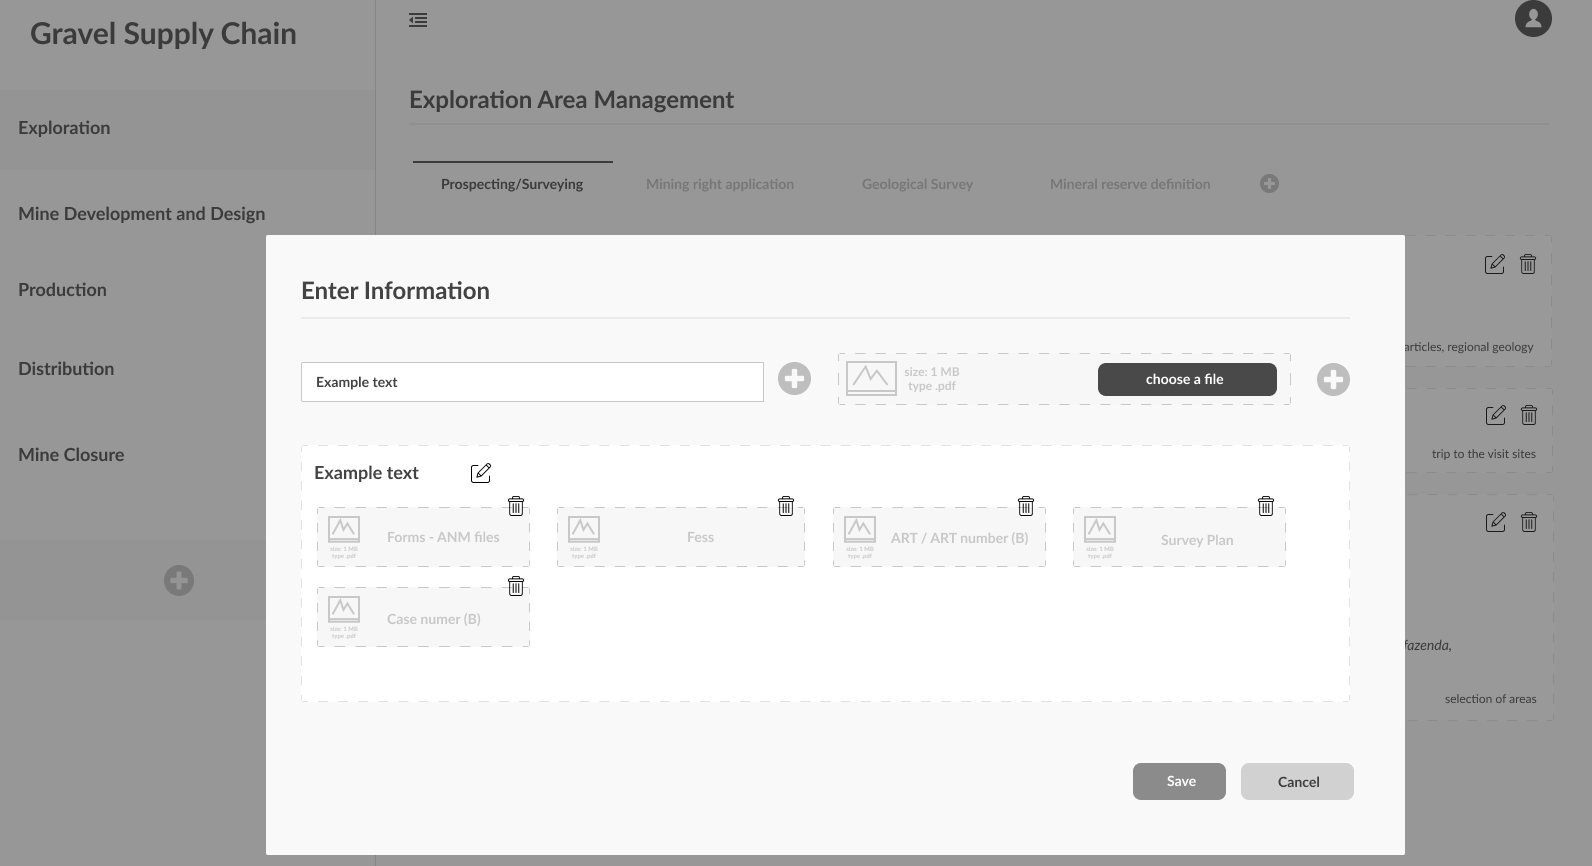
\includegraphics[scale=0.265]{images/frontend02.png}
\caption{SCM Configuration page}
\label{fig:frontend02}
\end{center}
\end{figure*}


Data storage is a general term for archiving data in electromagnetic or other forms for use by a computer or device. Different types of data storage play different roles in a computing environment. In addition to forms of hard data storage, there are now new options for remote data storage, such as cloud computing, and blockchain that can revolutionize the ways that users save and access data.  

Árion uses three applications as data storages: Blockchain, Cloud filesystem and relational database better detailed on next subsections. Blockchains grow continuously because of the amount of data and code in them, which is unchanging. Therefore, an important design decision is to choose which data and calculations to keep in and out of the chain.

\subsubsection{Filesystem}\label{sec:Filesystem}
A cloud file system is a tiered storage system that provides shared access to file data. Users can create, delete, modify, read and write files. All these actions generates a digital fingerprint (hash) information that is stored in the blockchain, separately from the original files or content, to keep consistency, traceability and auditability to the files.

A Cloud file sharing service gives multiple users simultaneous access to a cloud file data set. Cloud file sharing security is managed with user and group permissions, allowing administrators to tightly control access to shared file data.

\subsubsection{Database}\label{sec:Database}
A relational database is a set of formally described tables from which data can be accessed or reassembled in many different ways without having to reorganize the database tables. The standard user and application programming interface (API) of a relational database is the Structured Query Language (SQL). SQL statements are used both for interactive queries for information from a relational database and for gathering data for reports.

\subsubsection{Blockchain}\label{sec:DataStorageBlockchain}
The platform uses Blockchain to supply chain management tracking parts and service provenance, ensuring authenticity of goods, block counterfeits and reducing conflicts. This usually involves a limited and known number of actors, suggesting use of a permissioned Blockchain, that is, a Blockchain where all nodes must be allowed to be part of the system. To implement that, Hyperledger Fabric is used \cite{cachin2016architecture}. Hyperledger is an open source collaborative effort created to advance cross-industry Blockchain technologies. 

Hyperledger Fabric is an enterprise-grade permissioned distributed ledger framework for developing solutions and applications. Its modular and versatile design satisfies a broad range of industry use cases. It offers a unique approach to consensus that enables performance at scale while preserving privacy.

In context of Árion, the Blockchain module consists in smart contracts and the ledger. From the application developer’s perspective, a smart contract, together with the ledger, form the heart of a Hyperledger Fabric Blockchain system. Whereas a ledger holds facts about the current and historical state of a set of business objects, a smart contract defines the executable logic that generates new facts that are added to the ledger. 

\subsubsection{Chaincode}
Hyperledger Fabric implements smart contracts through chaincode. A chaincode is typically used by administrators to group related smart contracts for deployment, but can also be used for low level system programming of Fabric. These terms smart contract and chaincode are used interchangeably in a Hyperledger context. In general, a smart contract defines the transaction logic that controls the lifecycle of a business object contained in the world state. It is then packaged into a chaincode which is then deployed to a Blockchain network. So, smart contracts rule transactions, whereas chaincode rules how smart contracts are packaged for deployment.

Before businesses transact with each other, they must define a common set of contracts covering common terms, data, rules, concept definitions, and processes. Taken together, these contracts lay out the business model that govern all of the interactions between transacting parties. A smart contract defines the rules between different organizations in executable code. Applications invoke a smart contract to generate transactions that are recorded on the ledger.

Smart contracts have many APIs available to them. Critically, in all cases, whether transactions create, read, update or delete business objects in the world state, the Blockchain contains an immutable record of these changes.

